\chapter{Реалізація алгоритмів}             
            
    \section {Тестові дані}
            Для перевірки алгоритмів використовувались синтетичні набори даних. Була написана програма, що створює набір даних заданої форми. Утиліта зчитує із вказаного файла послідовно інформацію про центр групи об'єктів і дозволені відхилення від центру по кожній координаті та генерує вказану кількість об'єктів, розташованих випадковим чином у вказаних межах навколо центра. Задавши достатню кількість центральних точок і вибравши відповідні відхилення, можна отримати набір даних довільної форми. Зокрема, задавши центр групи приблизно посередині між усіма іншими точками, і досить великі відхилення по усіх координатах, можна досягнути ефекту шуму в даних ("зоряне небо"). Як і основна програма, утиліта написана на С++.
            
               
        \section {Програмне забезпечення}
            Для перевірки ефективності вищеописаних алгоритмів була створена їх програмна реалізація. У виборі мови програмування я керувався міркуваннями швидкодії та можливості контролю ресурсів комп'ютера. Вибір зупинився на С++. Реалізація являє собою консольну програму без графічного інтерфейсу, що зчитує дані з файла та зберігає у файлі результати кластеризації.
            
            %\begin{figure}
            %    \centering
            %    \includegraphics[scale=0.5]{chapters/03-software/Magister.png}
            %    \caption{Компонентна діаграма розробленого програмного забезпечення.}\label{fig:modules}
            %\end{figure}
            
            Створено об'єктно-орієнтовану модель для зберігання об'єктів вибірки. Для зберігання власне даних використовуються стандартні колекції STL. Де-юре STL не належить до стандарту мови С++, але де-факто усі сучасні поширені компілятори мають підтримку цеї бібліотеки. Перша версія програми включала об'єкт ,,DataContainer'', який містив асоціативний контейнер std::map, що дозволяв звертатись до обєктів вибірки по ідентифікатору. Кожен елемент вибірки був екземпляром класу Object, що містив std::vector вказівників на об'єкти класу Attribute. Кожен екземпляр Attribute містив числове значення відповідного атрибута та інформацію при присутність даного атрибута у відповідного об'єкта вибірки.
            
            Реалізовано також абстрактний клас AbstractMetric, який відповідав метриці простору. Архітектура програми дозволяє реалізувати довільну метрику простору. Таким чином при реалізації власне алгоритму кластеризації стало можливим абстрагуватись від типу метрики за допомогою механізму поліморфізму, доступного у С++. На даний момент із метрик реалізовано найпопулярнішу евклідову метрику.
            
            Написання програми відбувалось у текстовому редакторі vim. Для компіляції програми обрано компілятор gcc. Відлагодження програми відбувалось за допомогою набору інструментів gdb. Відслідковування витрат пам'яті та профілювання програми здійснювалось за допомогою valgrind. При розробці використовувалась система контролю версій git.
            
            Запуски програми та заміри часу проводились на комп’ютері із двоядерним процесором Intel Pentium D з тактовою частотою 2.8 ГГц. На комп’ютері встановлено 3 Гб оперативної пам’яті типу DDRII, що працює на частоті 667 МГц.
            
            Компіляція виконувалась із вказанням -О3 в якості рівня автоматичної оптимізації, в конфігурації Release.
            
            \subsection{K-means}
            
                K-means --- ітераційний алгоритм, тому час його роботи залежить не лише від об’єму вхідних даних, а і від їх структури. Тому оцінити загальний час роботи алгоритму складно. Натомість будемо оцінювати швидкодію конкретної реалізації за часом виконання одної ітерації. 
                
                На кожній ітерації k-means здійснюється обчислення центроїди кожного кластера, та обчислення відстані від кожного об’єкта до кожної центроїди. Оскільки на кожній ітерації кожен об’єкт повинен увійти в кластер, сумарна складність обчислення центроїд не змінюється між ітераціями. Кількість центроїд, очевидно, рівна кількості кластерів, тому час пошуку найближчої центроїди також залишається незмінним. Таким чином, час виконання ітерації на протязі усієї роботи алгоритму не змінюється. Це підтверджується графіком на рис.~\ref{fig:kmeans_linear}. Цей же графік ілюструє вплив розмірності простору та заданої кількості кластерів на час роботи ітерації. Розмірність простору впливає на складність обчислення відстані між об’єктами. на кожній ітерації для кожного об’єкта потрібно знайти найближчу центроїду. Кількість центроїд дорівнює кількості кластерів, тому остання прямо впливає на складність цього кроку.
                
                \begin{figure}
                    \centering
                    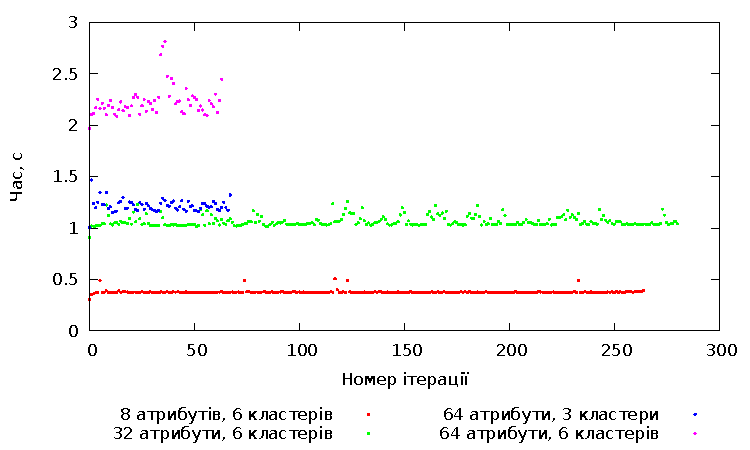
\includegraphics[scale=1.3]{kmeans_iteration_linear.pdf}
                    \caption{Графік залежності часу виконання ітерації k-means від її номера}\label{fig:kmeans_linear}
                \end{figure}
                
                На вхід алгоритму подавались три схожі синтетичні набори даних. Об’єкти в кожному з них розташовуються випадковим чином всередині n-вимірного куба з центром в початку координат та довжиною сторони, що дорівнює 2. Кількість об’єктів у кожному наборі --- 100000. Ці набори даних містили відповідно об’єкти з 8-вимірного, 32-вимірного та 64-вимірного просторів. Ці набори алгоритм повинен був розбити на 3 та 6 кластерів.
                
                \begin{figure}
                    \centering
                    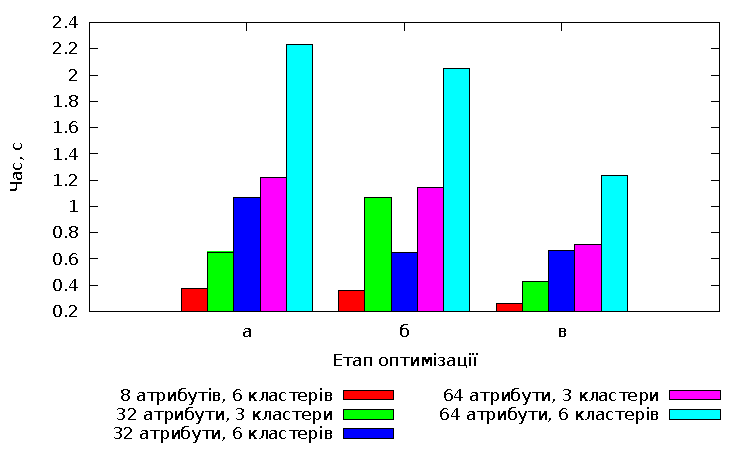
\includegraphics[scale=1.3]{kmeans_iteration_average.pdf}
                    \caption{Середній час виконання ітерацій k-means}\label{fig:kmeans_average}
                \end{figure}
                
                Рис.~\ref{fig:kmeans_average} показує середній час виконання ітерації k-means для різних вхідних даних. Рис.~\ref{fig:kmeans_average}, \emph{а} ілюструє роботу k-means у первинному вигляді. Рис.~\ref{fig:kmeans_average}, \emph{б} показує час роботи алгоритму після переходу на числа одинарної точності. Як бачимо, ця зміна суттєво вплинула лише на варіант запуску, що вимагав найбільше обчислень.
                
                Профілювання показало, що вибрана структура даних спричиняє великі втрати. За задумом, кожен екземпляр класу Object містив вектор екземплярів класу Attribute. Клас Attribute містив значення відповідного атрибуту та деяку додаткову інформацію (зокрема, дані про те, чи цей атрибут відомий із вхідного масиву). Це дозволяло легко розширити програму, додавши до неї функціонал передбачення даних, яких бракує у вибірці.
                
                За результатами профілювання від цеї структури довелось відмовитись. Замість вектора об’єктів використано динамічний масив чисел. Швидкість роботи k-means у такому випадку показано на рис.~\ref{fig:kmeans_average}, \emph{в}. Можна бачити, що така модифікація відчутно  зменшила час кожної ітерації.
                
            \section{DBSCAN}
                У DBSCAN кількість ітерацій рівна кількості об’єктів. На кожній ітерації вибирається один з об’єктів вибірки та обчислюються відстані від нього до усіх інших об’єктів вибірки. Таким чином, складність обчислень не змінюється між ітераціями. Проте, на відміну від k-means, залежно від результатів обчислень в ітерації можуть проводитись додаткові дії (такі як, наприклад, додавання сусідів об’єкта до списку об’єктів для подальшого аналізу). За рахунок додаткових операцій із пам’яттю ця особливість впливає на час роботи алгоритму. Відхилення від середнього значення часу виконання ітерації спостерігались в обидва боки (в менший бік, якщо в об’єкта немає достатньої кількості сусідів, і ніяк не впливає на список об’єктів для розгляду, і в більший, якщо об’єкт додає своїх сусідів до списку розгляду). Максимальний розмір відхилення --- 20\% від часу виконання ітерації.
                
                \begin{figure}
                    \centering
                    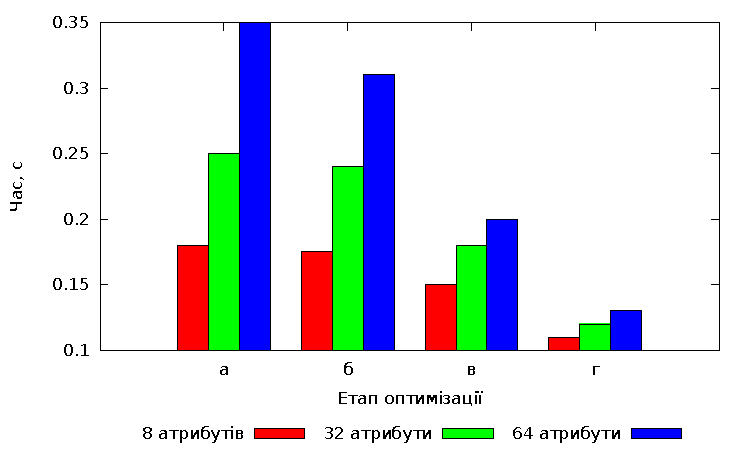
\includegraphics[scale=1.3]{dbscan_compare.pdf}
                    \caption{Середній час виконання ітерацій DBSCAN}\label{fig:dbscan_compare}
                \end{figure}
                
                На вхід алгоритму подавався той самий масив даних, що і для k-means. На рис.~\ref{fig:dbscan_compare} вказано середній час ітерації для кожного проведеного етапу оптимізації. На рис.~\ref{fig:dbscan_compare}, \emph{а} зображено час виконання одної ітерації для початкової версії алгоритму. Рис.~\ref{fig:dbscan_compare}, \emph{б} показує час виконання одної ітерації після переходу від чисел із подвійною точністю до чисел одинарної точності. Як і у випадку k-means, цей перехід мав суттєвий вплив лише на час обробки даних великої розмірності. Наступна група, рис.~\ref{fig:dbscan_compare}, \emph{в}, показує час виконання одної ітерації алгоритму після відмови від складної структури доступу до атрибутів об’єктів. Знову, аналогічно до k-means, цей перехід суттєво прискорив роботу алгоритму. Важливо звернути увагу на рис.~\ref{fig:dbscan_compare}, \emph{г}. Це --- результат оптимізації, що полягає у покращенні роботи з пам’яттю. Ця зміна призвела до зникнення залежності між кількістю близьких сусідів в об’єкта, що розглядається на певній ітерації, та часом виконання цеї ітерації. Такого покращення вдалось досягнути, відмовившись від деяких фактично зайвих операцій з пам’яттю.
                
            \subsection{UPGMA}
                UPGMA на кожній ітерації потребує матриці відстаней між усіма об’єктами вибірки. 
